% 0495(본책 91쪽) — □ABCD 와 두 대각선, ∠BAD=115°, ∠ABD=x(색칠), ∠ACB=40°. 다시 그림.
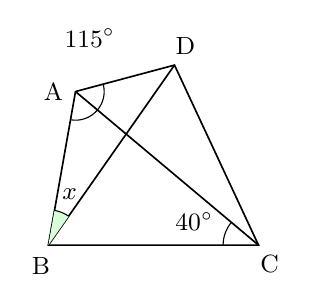
\begin{tikzpicture}[scale=1.40, line width=0.6pt]
  \draw (-0.707,0.843) -- (-0.953,-0.550) -- (0.953,-0.550) -- (0.191,1.083) -- cycle;
  \draw (-0.707,0.843) -- (0.953,-0.550);
  \draw (-0.953,-0.550) -- (0.191,1.083);
  \draw[line width=0.4pt] (-0.752,0.587) arc[start angle=-100.000, end angle=15.000, radius=0.260];
  \node[font=\small, inner sep=0.5pt] at (-0.578,1.326) {$115^\circ$};
  \fill[green!15] (-0.953,-0.550) -- (-0.769,-0.288) arc[start angle=55.000, end angle=80.000, radius=0.320] -- cycle;
  \draw[line width=0.4pt] (-0.769,-0.288) arc[start angle=55.000, end angle=80.000, radius=0.320];
  \node[font=\small, inner sep=0.5pt] at (-0.761,-0.088) {$x$};
  \draw[line width=0.4pt] (0.707,-0.344) arc[start angle=140.000, end angle=180.000, radius=0.320];
  \node[font=\small, inner sep=0.5pt] at (0.370,-0.338) {$40^\circ$};
  \node[font=\small, inner sep=1.5pt] at (-0.907,0.843) {A};
  \node[font=\small, inner sep=1.5pt] at (0.291,1.256) {D};
  \node[font=\small, inner sep=1.5pt] at (-1.021,-0.738) {B};
  \node[font=\small, inner sep=1.5pt] at (1.053,-0.723) {C};
\end{tikzpicture}
